% Template for a Thesis
%
% thesis.tex
%
% This is the central document.

% general settings
% Template for a Thesis
%
% settings.tex
%
% Here general setting are made

\documentclass[%
	a4paper,%							A4 paper
	oneside,%							oneside (left and right margin are equal
	bibliography=totoc,%	add the bibliography to the table of contents
	%listof=totoc,%				add the list of figures and list of tables to the table of contents
	numbers=noenddot,%		no dot at the end of heading numbers (see the comment below)
	headsepline,%					line after the page head
	footsepline,%					line before the page foot
	headings=small,%			smaller headings
	11.5pt,%								font size
]{scrreprt}

% According to the famous German dictionary 'Duden'
% (see https://en.wikipedia.org/wiki/Duden), the following rules apply:
% If only Arabic numbers are used to number the sections, no end dot is used.
% If also Roman numbers or letters are used to number the sections, a terminatory dot shall be placed.
% The KoMA script tries to determine the used numbering 
% scheme in its default setting and applies the corresponding rule.
% (This information is saved in the .aux file,
% therefore a second LaTeX run might be necessary.)

% package for english language
\usepackage[english]{babel}

% input encoding
\usepackage[utf8]{inputenc}

% output font encoding
\usepackage[T1]{fontenc}

% output font
\usepackage{lmodern}

% microtypographical improvements
\usepackage{microtype}

% more options for tables
\usepackage{array}

% nicer tables
\usepackage{booktabs}

% package to check for pdf mode
\usepackage{ifpdf}

% package for graphics
% the formats png, pdf, jpg are permitted
\usepackage{graphicx}
% default path for figures
\graphicspath{{figures/}}
% default file extensions for figures
\ifpdf
	% for pdf output
	\DeclareGraphicsExtensions{.pdf,.jpg,.png}
\else
	% for html output
	\DeclareGraphicsExtensions{.png,.jpg}
\fi

% package to allow for dots in filenames
\usepackage{grffile}

% package for the "drawing" of figures
\usepackage{tikz}

% package for rendering plots using TikZ
\usepackage{pgfplots}
% always use the newest version
\pgfplotsset{compat=newest}
% format and size template for two plots side-by-side
\pgfplotsset{
	scriptsize/.style={
		width=4.5cm,
		height=,
		legend style={font=\scriptsize},
		tick label style={font=\scriptsize},
		label style={font=\footnotesize},
		title style={font=\footnotesize},
		every axis title shift=0pt,
		max space between ticks=15,
		every mark/.append style={mark size=7},
		major tick length=0.1cm,
		minor tick length=0.066cm,
	},
}
% new format setting for a usual coordinate system
\pgfplotsset{
	coordinatesystem/.style={
		axis x line=middle,
		axis y line=center,
		xmajorgrids=false,
		ymajorgrids=false,
		legend style={draw=none},
	},
}
% align legends entries to the left
\pgfplotsset{legend cell align=left}
% draw a main grid
\pgfplotsset{xmajorgrids}
\pgfplotsset{ymajorgrids}
% number of minor ticks between two major tickmarks
%\pgfplotsset{minor x tick num={3}}
%\pgfplotsset{minor y tick num={3}}
% draw a minor grid
%\pgfplotsset{xminorgrids}
%\pgfplotsset{yminorgrids}
% scale only the axis using a certain width and height
\pgfplotsset{scale only axis}
% define colors like in MATLAB (version R2014a and earlier)
%\definecolor{matlab1}{rgb}{0,0,1}
%\definecolor{matlab2}{rgb}{0,0.5,0}
%\definecolor{matlab3}{rgb}{1,0,0}
%\definecolor{matlab4}{rgb}{0,0.75,0.75}
%\definecolor{matlab5}{rgb}{0.75,0,0.75}
%\definecolor{matlab6}{rgb}{0.75,0.75,0}
%\definecolor{matlab7}{rgb}{0.25,0.25,0.25}
% define colors like in MATLAB (since version R2014b)
% see: https://de.mathworks.com/help/matlab/graphics_transition/why-are-plot-lines-different-colors.html
% The RGB values can also be read out via:
% >> figure;
% >> get(gca,'defaultAxesColorOrder');
% Thanks to Thomas Aab for the update.
\definecolor{matlab1}{rgb}{0,0.4470,0.7410}
\definecolor{matlab2}{rgb}{0.8500,0.3250,0.0980}
\definecolor{matlab3}{rgb}{0.9290,0.6940,0.1250}
\definecolor{matlab4}{rgb}{0.4940,0.1840,0.5560}
\definecolor{matlab5}{rgb}{0.4660,0.6740,0.1880}
\definecolor{matlab6}{rgb}{0.3010,0.7450,0.9330}
\definecolor{matlab7}{rgb}{0.6350,0.0780,0.1840}
% define a color cycle list like in MATLAB
\pgfplotscreateplotcyclelist{matlab}{
	{matlab1,solid},
	{matlab2,dashed},
	{matlab3,dashdotted},
	{matlab4,dotted},
	{matlab5,densely dashed},
	{matlab6,densely dashdotted},
	{matlab7,densely dotted}%this prevents an error
}
% use the earlier defined color list
\pgfplotsset{cycle list name=matlab}
% use the standard color list of pgfplots
%\pgfplotsset{cycle list name=color list}
% use only grayscale lines
%\pgfplotsset{cycle list name=linestyles}
% use a line width of 1pt
\pgfplotsset{every axis plot/.append style={line width=1pt}}
% use a comma as the dot separator for german documents
\addto\extrasngerman{\pgfplotsset{/pgf/number format/.cd,set decimal separator={{{,}}}}}
% use a half space as the 1000 separator
\pgfplotsset{/pgf/number format/.cd,1000 sep={\,}}

% package for subfigures in one figure
\usepackage{subfig}

% mathematical symbols
\usepackage{amsmath}
\usepackage{amssymb}

% package to change the line spacing
\usepackage{setspace}
% use onehalf line spacing
\onehalfspacing
% set headlines in single spacing
% see http://www.mrunix.de/forums/showthread.php?p=356306
\addtokomafont{pageheadfoot}{\linespread{1}\selectfont}

% package to rotate text
\usepackage{rotating}

% package for colors
\usepackage{color}

% package for better quotes
\usepackage{csquotes}

% package for better citations
\usepackage{cite}

% package to not account for citations in the toc, lof or lot during the numbering
\usepackage{notoccite}

% package for underscores
\usepackage[normalem]{ulem}

% package for SI units
\usepackage[binary-units]{siunitx}
% options
% real fractions
\sisetup{per-mode=fraction,mode=math}
% decimal marker in dependence from the language
\addto\extrasngerman{\sisetup{output-decimal-marker={,}}}
\addto\extrasenglish{\sisetup{output-decimal-marker={.}}}
% range phrase in dependence from the language
\addto\extrasngerman{\sisetup{range-phrase={ bis~}}} 
\addto\extrasenglish{\sisetup{range-phrase={ to~}}}

% define new mathematical functions
\DeclareMathOperator{\arcosh}{arcosh}

% differential operator (small upright d)
\newcommand*{\diff}{\mathop{}\!\mathrm{d}}

% redefine the exponential function
\DeclareMathOperator{\e}{e}
\renewcommand{\exp}[1]{\e^{#1}}

% write indices upright (in Roman)
\newcommand{\ind}[1]{\mathrm{#1}}

% a period in a math environment
\newcommand{\period}{\,\text{.}}
% a comma in a math environment
\newcommand{\comma}{\,\text{,}}

% magnitude or absolute value
\newcommand{\abs}[1]{\left| #1 \right|}

% mean value or average value
\newcommand{\mean}[1]{\left\langle #1 \right\rangle}

% package for nice fractions in the text mode
\usepackage{xfrac}

% set page margin with the geometry package
\usepackage[margin=2.5cm]{geometry}

% set the hyphenation for certain words
\hyphenation{op-tic-al net-works semi-con-duc-tor}

% package for a notation/nomenclature
\usepackage{nomencl}
\makenomenclature

% package for a list of abbreviations
% refer to: http://www.ctan.org/tex-archive/macros/latex/contrib/acronym/acronym.pdf
\usepackage{acronym}

% always try to place figures and tables 'here'
\makeatletter
\renewcommand{\fps@figure}{htbp}
\renewcommand{\fps@table}{htbp}
\makeatother

% portion of floating figures and tables at the top of a page
% default value: 0.7
\renewcommand{\topfraction}{0.8}

% portion of floating figures and tables at the bottom of a page
% default value: 0.3
\renewcommand{\bottomfraction}{0.33}

% one of these values (\topfraction and \bottomfraction) has to be larger than \floatpagefraction

% portion of floating figures and tables for a new page only for floating objects
% default value: 0.5
\renewcommand{\floatpagefraction}{0.66}

% portion of a page for floating objects that is reserved for text
% default value: 0.2
\renewcommand{\textfraction}{0.10}

% numbering till subsection in the text
\setcounter{secnumdepth}{2}

% numbering till subsection in the table of contents
\setcounter{tocdepth}{2}

% new line after paragraph
% siehe http://tex.stackexchange.com/questions/40943/new-line-and-no-indent-after-paragraph
\makeatletter
\renewcommand\paragraph{\@startsection{paragraph}{4}{\z@}%
  {-3.25ex \@plus -1ex \@minus -0.2ex}%
  {0.01pt}%
  {\raggedsection\normalfont\sectfont\nobreak\size@paragraph}%
}
\makeatother

% package for an intelligent space character
\usepackage{xspace}

% abbrevations
\newcommand{\eg}{e.\,g.\xspace}
\newcommand{\ie}{i.\,e.\xspace}

% hyperref package for links in the document
\usepackage[
	pdftitle={Degree Thesis},
	pdfauthor={John Doe},
	pdfcreator={MiKTeX, LaTeX with hyperref and KOMA-Script},
	pdfsubject={Guidance on the Preparation of Degree Theses},
	pdfkeywords={Structure, Contents, Layout},
	pdfstartview={Fit}]{hyperref}

% listings for code listings
\usepackage{listings}
\usepackage{pythonhighlight}
% end of file

\begin{document}

% new lengths for a harmonized width of the plots
\newlength{\plotwidth}
\setlength{\plotwidth}{0.7\columnwidth}
\newlength{\plotheight}
\setlength{\plotheight}{0.66\plotwidth}
\newlength{\semiwidth}
\setlength{\semiwidth}{0.35\columnwidth}
\newlength{\semiheight}
\setlength{\semiheight}{0.66\semiwidth}

% the titlepage
\pagenumbering{alph}
\pagestyle{empty}
% Template for a Thesis
%
% titlepage.tex
%
% Here the titlepage is generated.

\begin{titlepage}
	\begin{center}
		\normalsize
		Ludwig-Maximiliams-Universität München \\
		Center for information and language processing (CIS)  \\
		Faculty of language and literature sciences \\
		\vspace{1cm} % vertical space
		\huge
		Master thesis \\
		\vspace{1.5cm}
		
\includegraphics[width=12cm]{figures/lmu_logo.png} \\ % insert the university logo
		\vspace{1cm}
		\Large
		This is the unknown title \\
		of my master thesis \\
		\vspace{1cm}
		\tiny Version 0, 9 June 2020
	\end{center}
	\normalsize
	\vfill % variable vertical space
	\begin{labeling}{submitted: }
		\item[submitted:] \today
		\item[by:] Ane Berasategi
		\item[supervisor:] Masoud Jalil Sabet
		\item[supervisor:] Hinrich Schütze
	\end{labeling}
\end{titlepage}

% end of file


% the preface
\pagenumbering{roman}
\pagestyle{plain}
% Template for a Thesis
%
% abstract.tex
%
% Abstract

\section*{Abstract}

An \emph{abstract} is a brief summary of a research article, thesis, review, 
conference proceeding or any in-depth analysis of a particular subject or 
discipline, and is often used to help the reader quickly ascertain the paper's 
purpose. When used, an abstract always appears at the beginning of a manuscript, 
acting as the point-of-entry for any given academic paper or patent application. 
Abstracting and indexing services for various academic disciplines are aimed at 
compiling a body of literature for that particular subject~\cite{wiki:abstract_en}.

% end of file

-% Template for a Thesis
%
% task.tex
%
% Task of the thesis in the original

\section*{Task of the Thesis in the Original:}

%\begin{center}
%	\includegraphics[width=0.95\textwidth]{task}
%\end{center}

% end of file
% Template for a Thesis
%
% declaration.tex
%
% Declaration

\section*{Declaration by the candidate}

I hereby declare that this thesis is my own work and effort and that it has not been submitted anywhere for any award. Where other sources of information have been used, they have been marked.

\bigskip

The work has not been presented in the same or a similar form to any other testing authority and has not been made public.

\bigskip

I hereby also entitle a right of use (free of charge, not limited locally and for an indefinite period of time) that my thesis can be duplicated, saved and archived by the Ludwig Maximilians University (LMU) or any commissioned third party (\eg \emph{iParadigms Europe Limited}, provider of the plagiarism-detection service \enquote{Turnitin}) exclusively in order to check it for plagiarism and to optimize the appraisal of results.

\bigskip

Munich, \today

% end of file

% the table of contents and the lists of figures and tables
\pagenumbering{arabic}
\pagestyle{headings}
\tableofcontents
% Template for a Thesis
%
% notation.tex
%
% Notation/nomenclature

% set the correct headline
\markboth{\nomname}{\nomname}
% print the nomenclature with 2 cm distance between the symbol and the explanation
\printnomenclature[2cm]

% general notations
\nomenclature[#1]{$a$,$A$}{scalar, also complex valued}
\nomenclature[#2]{$\vec{a}$,$\vec{A}$}{vector, also complex valued}

% end of file
% Template for a Thesis
%
% acronyms.tex
%
% List of Acronyms

\chapter*{List of Acronyms}

\begin{acronym}[PDF~]
 \acro{NLP}{Natural language processing}
\end{acronym}

% end of file
\listoffigures
\listoftables

% the actual content
% Template for a Thesis
%
% 1-introduction.tex
%
% Introduction

\chapter{Introduction}\label{sec:introduction}

Natural language processing, NLP, is the task of processing natural language, transforming it, obtaining information from it, classifying it, translating it, and many other tasks. It is closely related to NLU, natural language understanding, which seeks to more theoretically understand the meaning of language. It could be said that linguistics is more involved in NLU, whereas computer science, algorithms and programming are the backbone of NLP.

There has been great progress in NLP since around 2017 until the time of writing, 2020, mostly driven by computational advances. Pre-2017 NLP mostly used convolutional or recurrent neural networks, built them from scratch with hundreds of thousands of hyperparameters and trained them on CPUs locally. The datasets used for these models were comparable in size with the models. In 2017, Vaswani et al~\cite{vaswani2017attention} introduced a model neural network architecture, Transformers, that removed any sequentiallity and focused solely on attention. This architecture is very powerful and soon thereafter, BERT~\cite{devlin2018bert} was introduced, which enabled the pre-training of deep bidirectional Transformers. BERT is very computationally expensive and requires intensive training, which is why the authors published pre-trained weights on many NLP tasks that users could later fine tune for their own applications. This introduced the era of pre-training, when users do not train models from scratch anymore and use huge, already pre-trained models. Anyone who wishes to train state-of-the-art models at the time of writing requires very powerful GPUs or even TPUs, which are only available to large organizations given their enormous cost, and several days or even weeks of training, which produces a gigantic energy consumption, as a study from 2019 suggests~\cite{strubell2019energy}. Bigger datasets, bigger models, better embeddings have been trained and published, and they are more power hungry every year. Neural networks, especially the ones being used nowadays, given their size, require vast amounts of data in order to process and adapt their billions of hyperparameters.

It could be said that most of the advances in the past 3-5 years have been computational, and not so much linguistic. The deep learning pipeline has barely changed. First of all, a corpus is read and parsed. Then, embeddings are applied to the parsed corpus and fed to the neural network. This in turn is trained for a number of epochs, the weights typically saved for posteriority, and then the model is evaluated against a test set. Independently of the size or architecture of the neural network, the training time and the relatively new addition of embeddings, the main idea of machine learning has not changed.

This thesis does not introduce any new parameter in the main pipeline, but rather focuses on the corpus-embeddings step and explores how the corpus is parsed so that the embeddings are optimally applied to it. The definition and usage of embeddings is explained in the literature review section of this thesis, but in broad terms, embeddings are a mapping between characters and numbers. Computers cannot work with pictures, audio or language, they only process numbers, which is why for all data types, they first need to be transformed into numbers. How to make this transformation depends at great extent on the type of data: for instance, sequentiallity is very important in audio and language. An utterance or word generally loses its meaning when it is displaced in time. In images, however, the important metric is knowing which pixels are close to which pixels in order to get a meaning out of a group of pixels. For language, the numbers fed to the computer should not just be numbers: they should encode meaning. Embeddings map any text to a fixed size vector, say 50 numbers one after another, in a way that the numbers of similar words are also very similar. The embedding vector of gray and black are therefore very similar.

Historically, embeddings have been applied to words. That is, the word \emph{black} has the same embedding vector regardless of the context, where it might be used to talk about colors, the sky, or race. This creates some problems since words can have different meanings depending on the context. After BERT, the chosen method has been subword embeddings, applying the mapping to parts of the word instead of the whole. For example, the word \emph{extraterrestrial} would be first segmented into \emph{extra-terrestr-ial}, and each unit would get assigned a different embedding. There have been many methods to obtain this segmentation, the most popular one being BPE~\cite{sennrich2015neural}.

This thesis has explores he details of the BPE algorithm, coded it from scratch to deeper understand it, and replicated its results. Some improvements have been done to parts of the algorithm used in the original paper, which are presented in this thesis. A newer version of BPE, published in 2019, has also been explored, analyzed, coded and its results replicated. Some of the hyperparameters used in this method have been tweaked and its performance slightly improved. BPE-dropout~\cite{provilkov2019bpedropout} improves the performance of BPE, which has been shown in this thesis for English-German and also for other language pairs, confirming its consistency. Moreover, the most novel addition of this thesis, is applying BPE without any word boundaries.

In English and Indo-European languages, the smallest unit in language that preserves meaning is the word. Given a sentence with 5 words, it is possible to assign one meaning to each word, and obtain the meaning of the sentence by uniting the meanings of the words. But in other languages where not words, but symbols are used, the whitespace between words does not have the same defining meaning as in Indo-European languages, and perhaps it would make sense to apply embeddings to a group of whitespace-separated symbols.

As a result, this thesis extends BPE to perform also in the case where multiple-word units are allowed. The evaluation method chosen to observe the performance of BPE is not prepared to deal with multi-word units, and the thesis shows that the performance is lower in this case. However, for a specific combination of hyperparameters, the results are comparable to those of BPE using whitespace as word boundary. Finally, it is also shown that BPE-dropout outperforms BPE also in this new case of no word boundaries.

% Template for a Thesis
%
% 2-goals.tex
%
% Goals

\chapter{Goals of the thesis}

The goal of this thesis has been primarily to analyse the BPE algorithm, as a way to tokenize raw text and as opposed to other tokenization methods such as word tokenization, or other subword tokenizations. After reading this thesis the reader should have no doubts as to how the BPE algorithm works, given the extensive array of examples and codes that are presented throughout the thesis. This thesis also aims to replicate the BPE algorithm and obtain satisfactory performance results.

In order to evaluate the performance of the BPE algorithm, an alignment method from statistical machine translation is transferred into this scenario, to compare the difference between aligning words and subword units.

An additional goal is to analyse, understand and replicate an improvement over BPE called BPE dropout. The intricancies of the algorithm improvement, the motivation stemming from some of BPE's drawbacks will be explained, and examples and codes included as well. By iterating on some of the hyperparameters used to obtain BPE dropout results, this thesis will atempt to improve BPE dropout's results.

This thesis will also intend to improve the original BPE learning algorithm, making a dramatic improvement in performance. Furthermore, a new paradigm to obtain BPE units will be presented, namely removing the space boundary between words to admit creating BPE units among different words. This will be integrated into the algorithm, so that the end user can choose which mode to use, either the traditional space separated version employed in the BPE and BPE dropout paper, or the new one. 

The pipeline will be automated and easy to tweak in the sense that by changing some parameters in a global file, such as dropout rate, number of merges, space mode on or off, etc. the pipeline will automatically adapt to the specific scenario.
% Template for a Thesis
%
% 3-tokenization.tex
%
% Tokenization

\chapter{Tokenization}\label{sec:tokenization}

Tokenization is the first major step in language processing. Once the corpus is obtained, before starting to process the text, because we're dealing with language, we want to understand the meaning of the text. \textbf{Tokens} in the language have a semantic meaning, be it words, phrases, symbols or other elements, whereby a meaning is assigned to each token. Tokenization is the process of breaking a stream of text up into tokens.~\cite{manning2008introduction}

The way to tokenize heavily depends on the task afterwards. Some applications might require different tokenization algorithms. Nowadays, most deep learning architectures in NLP process the raw text at the token level and as a first step, create embeddings for these tokens, which will be explained in more detail in the following sections. In short, the type of tokenization depends on the type of embedding. There are several, explained further in the following sections, and each has its advantages and drawbacks.

\paragraph{What is a token?}

A token is an instance of a sequence of characters in some particular document that are grouped together as a useful semantic unit for processing. Here is an example of tokenization.

\begin{quote}
    Input: I ate a burger today, and it was good.\\
    Output: ['I', 'ate', 'a', 'burger', 'today', 'and', 'it', 'was', 'good']
\end{quote}

In this example, the way to obtain tokens looks simple: just locate word boundaries, split by whitespace and get the symbols, and remove the punctuation marks, since punctuation marks have no definite meaning. However, this is not always the case.

\paragraph{How to deal with punctuation marks?}

Each language has its own set of tricky cases, for example in English what is the correct approach when dealing with apostrophes for possession and contractions? For example words like \emph{aren't}, \emph{Sarah's} and \emph{O'Neill}. Because of this, it is imperative to know the language of the text to be tokenized. \textit{Language identification} is the task of identifying the language of the input text. From the initial k-gram algorithms used in cryptography (Konnheim, 1981), to more modern n-gram methods (Dunning, 1994) have been used. Once the language is known, we can follow the rules for each case and deal with punctuation marks appropriately.

\paragraph{Other types of tokens}

Additionaly, tokens can be either characters or \textbf{subwords}. For example, the word \emph{smarter}:

\begin{quote}
    Sentence: the smarter computer
    Word: the, smarter, computer\\
    Word without word boundaries: the smart, er comput, er\\
    Character tokens: t-h-e, s-m-a-r-t-e-r, c-o-m-p-u-t-e-r\\
    Subword tokens: the, smart-er, comput-er
\end{quote}

The major question in the tokenization phase is: \textit{what are the correct tokens to use?}. The following section explores these 4 types of tokenization methods and delves into the algorithms and code libraries available.


\section{Motivation}



\section{Tokenization algorithm types}

Tokenization can be performed on word, character, or subword level.

\subsection{Word level tokenization}

Conceptually, splitting on whitespace can also split an element which should be regarded as a single token. This is mostly the case with names, borrowed foreign phrases, and compounds that are sometimes written as multiple words. In the case of information retrieval, splitting tokens on spaces can cause bad retrieval results. This problem can be mitigated by asking the user to write such words with a hyphen between them, but this requires user training.~\cite{manning2008introduction}.

\paragraph{Word embeddings}

As stated before, the goal of tokenization is to split the text into units with meaning. Typically, each token is assigned an embedding vector: Mikolov et al. \cite{mikolov2013efficient} introduced word2vec in 2013, as a way of encoding a word in a fixed-size vector of numbers that, viewed abstractly in its N dimensions, that word is close to similar words. As a simple example: 

\begin{quote}
    Word: smart, embedding: [2, 3, 1, 4]\\
    Word: intelligent, embedding: [2, 3, 2, 3]\\
    Word: stupid, embedding: [-2, -4, -1, -3]
\end{quote}

The embedding numbers are just as an example, to illustrate the distances between words. For example, \emph{smart} and \emph{intelligent} have a distance of 2, since the last 2 numbers in the vector differ by one respectively. If this was plotted in a 4 dimensional space, these words would be very close together. On the other hand, \emph{stupid} is almost the opposite of \emph{smart}. The distance in this case is much higher. In the plot, these words would be very far apart.

Thus, with word embeddings, a sentence is transformed into a sequence of embedding vectors, which is very useful for NLP tasks. Word embeddings have some drawbacks however. In many cases, a word can have more than one meaning: \emph{well}, for example, can be used in these 2 scenarios.

\begin{quote}
    I 'm doing quite well.\\
    The well was full of water.
\end{quote}

In the first case, well is an adverb while in the second it's a noun. \emph{well}'s embedding will probably be a mixture of the two, since word embeddings don't generalize to homonyms.

Another drawback is that if word embeddings are created with a certain vocabulary size, and then a new word arrives which isn't present in the vocabulary, because it's a foreign word, or a misspelled word, it will be given an unknown <UNK> embedding, that will be the same for all unknown words.

These problems are not to be mistaken with tokenization problems, tokenization is merely a way to an ends, they're mostly used to create embeddings. And if embeddings from word tokens are problematic, the tokenization method is changed in order to create different tokens, in order to create other types of embeddings.


Word level tokenization was the first type that was created, and is also the most commonly used tokenization algorithm. It splits a piece of text into individual words based on a specific delimiter, usually whitespace ' ' or other punctuation signs. Depending on this delimiter, different word-level tokens are formed.

\subsubsection{Word level algorithms}

Pretrained Word Embeddings such as Word2Vec and GloVe comes under word tokenization.

https://medium.com/@zafaralibagh6/simple-tutorial-on-word-embedding-and-word2vec-43d477624b6d
https://www.analyticsvidhya.com/blog/2017/06/word-embeddings-count-word2veec/
https://towardsdatascience.com/introduction-to-word-embedding-and-word2vec-652d0c2060fa

split(), regex, nltk, spacy, keras, gensim

https://www.analyticsvidhya.com/blog/2019/07/how-get-started-nlp-6-unique-ways-perform-tokenization/

1. Penn TreeBank:

It is a rule-based tokenization method that separates out clitics ( words that normally occur only in combination with another word, for example in I’m), keeps hyphenated words together, and separates out all punctuation.

It is mainly used with treebanks http://faculty.washington.edu/fxia/lsa2011/slides/intro\_to\_treebanks.pdf released by Linguistic Data Consortium. https://www.ldc.upenn.edu/

\subsubsection{Word level drawbacks}

One of the major issues with word tokens is dealing with Out Of Vocabulary (OOV) words. OOV words refer to the new words which are encountered at testing. These new words do not exist in the vocabulary. Hence, these methods fail in handling OOV words.

But wait – don’t jump to any conclusions yet!

    A small trick can rescue word tokenizers from OOV words. The trick is to form the vocabulary with the Top K Frequent Words and replace the rare words in training data with unknown tokens (UNK). This helps the model to learn the representation of OOV words in terms of UNK tokens
    So, during test time, any word that is not present in the vocabulary will be mapped to a UNK token. This is how we can tackle the problem of OOV in word tokenizers.
    The problem with this approach is that the entire information of the word is lost as we are mapping OOV to UNK tokens. The structure of the word might be helpful in representing the word accurately. And another issue is that every OOV word gets the same representation

Another issue with word tokens is connected to the size of the vocabulary. Generally, pre-trained models are trained on a large volume of the text corpus. So, just imagine building the vocabulary with all the unique words in such a large corpus. This explodes the vocabulary!

This opens the door to Character Tokenization.
    
\subsection{Character level tokenization}

Character Tokenization splits apiece of text into a set of characters. It overcomes the drawbacks we saw above about Word Tokenization.

    Character Tokenizers handles OOV words coherently by preserving the information of the word. It breaks down the OOV word into characters and represents the word in terms of these characters
    It also limits the size of the vocabulary. Want to talk a guess on the size of the vocabulary? 26 since the vocabulary contains a unique set of characters

https://www.lighttag.io/blog/character-level-NLP/
https://github.com/fnl/segtok
https://github.com/fnl/syntok

\subsubsection{Character level algorithms}

\subsubsection{Character level drawbacks}

Character tokens solve the OOV problem but the length of the input and output sentences increases rapidly as we are representing a sentence as a sequence of characters. As a result, it becomes challenging to learn the relationship between the characters to form meaningful words.

This brings us to another tokenization known as Subword Tokenization which is in between a Word and Character tokenization.

\subsection{Subword level tokenization}

Subword Tokenization splits the piece of text into subwords (or n-gram characters). For example, words like lower can be segmented as low-er, smartest as smart-est, and so on.

Transformed based models – the SOTA in NLP – rely on Subword Tokenization algorithms for preparing vocabulary. Now, I will discuss one of the most popular Subword Tokenization algorithm known as Byte Pair Encoding (BPE).

\subsubsection{Subword level algorithms}

BPE, WordPiece, SentencePiece. since BPE is the basis of the thesis, it deserves a section in itself.

\subsubsection{Subword level drawbacks}

...


\subsection{Tokenization without word boundaries}

Since there are many possible segmentations of character sequences and given the complications of dealing with different languages and the intricancies of each, there is no foolproof and/or unique tokenization. Another approach has been to abandon word-based indexing, and do all indexing from just short subsequences of characters (character -grams), regardless of whether particular sequences cross word boundaries or not.

This can be specifically beneficial in some Asian languages, where an individual symbol can resemble a syllable rather than a word or letter,  most words are short (the most common length is 2 characters), and that, given the lack of standardization of word breaking in the writing system, it is not always clear where word boundaries should be placed.

Punctuations are rare in certain languages!!

Hence, at times, each character used is taken as a token in Chinese tokenization.

\section{BPE}

Byte Pair Encoding (BPE) is a widely used tokenization method among transformer-based models. BPE addresses the issues of Word and Character Tokenizers:

    BPE tackles OOV effectively. It segments OOV as subwords and represents the word in terms of these subwords
    The length of input and output sentences after BPE are shorter compared to character tokenization

BPE is a word segmentation algorithm that merges the most frequently occurring character or character sequences iteratively. Here is a step by step guide to learn BPE.

Steps to learn BPE

    Split the words in the corpus into characters after appending </w>
    Initialize the vocabulary with unique characters in the corpus
    Compute the frequency of a pair of characters or character sequences in corpus
    Merge the most frequent pair in corpus
    Save the best pair to the vocabulary
    Repeat steps 3 to 5 for a certain number of iterations

Example in https://www.analyticsvidhya.com/blog/2020/05/what-is-tokenization-nlp/

\subsection{Applying BPE to OOV words}

(see python code bpe\_10.py)

But, how can we represent the OOV word at test time using BPE learned operations? Any ideas? Let’s answer this question now.

    At test time, the OOV word is split into sequences of characters. Then the learned operations are applied to merge the characters into larger known symbols.

    – Neural Machine Translation of Rare Words with Subword Units, 2016

Here is a step by step procedure for representing OOV words:

    Split the OOV word into characters after appending </w>
    Compute pair of character or character sequences in a word
    Select the pairs present in the learned operations
    Merge the most frequent pair
    Repeat steps 2 and 3 until merging is possible

\subsection{BPE dropout}

\section{WordPiece}

Byte Pair Encoding falter outs on rare tokens as it merges the token combination with maximum frequency.

WordPiece Tokenization is almost similar to Byte Pair Encoding. The only difference lies in the way we merge up the tokens to produce new tokens. While in BPE, we use the max frequency of the new token for merging but in WordPiece, we also take in consideration the frequency of two tokens separately used for merging apart from the frequency of the new token. This means if we have 2 token A \& B, we will be calculated:

Score(A,B) = Frequency(A,B)/Frequency(A)*Frequency(B) and max value pair will be selected

This definitely has an edge over Byte Pair Encoding.

It might be the case that Frequency(‘so’,’ on’) is very high but their separate frequencies are also high, hence if using WordPiece , we won’t be merging ‘soon’ as the overall score might go low. Again if Frequency(‘Jag’,’gery’) might be low but if their separate frequencies are also low, we will merge to form ‘jaggery’.

4. Unigram Language Model:

Let’s see the below example:

Even if we merged ‘face’+’d’ over ‘no’+’d’, it doesn’t mean we won’t encounter ‘nod’ ever. It just means that the probability of ‘nod’ is lesser but not 0. But if we use WordPiece, we might miss this.

So, what do to now?

What we need is a model that provides us with the probability of different tokens that can be generated. This simply means if we get the word ‘nod’, we shall get probabilities for ‘no+d’, ‘n+od’,’ nod’ but with different probabilities given the case these tokens (no,d, n, od, nod) are given in the initial vocabulary.

Let’s explore the Unigram Language model now

Read more in https://medium.com/data-science-in-your-pocket/tokenization-algorithms-in-natural-language-processing-nlp-1fceab8454af

\section{{SentencePiece}}

See medium link from wordpiece section

% https://www.quora.com/NLP-What-does-it-mean-Tokenizing
% https://www.quora.com/Why-is-tokenization-important-in-NLP
% https://en.wikipedia.org/wiki/Lexical\_analysis#Tokenization

% Template for a Thesis
%
% 4-translation.tex
%
% Translation

\chapter{Translation}\label{ch:translation}

\section{Statistical machine translation (SMT)}

SMT is a machine translation approach where translations are generated based on statistical models, whose parameters are derived from the analysis of bilingual text corpora. It can be done with rule-based approaches in a supervised way, or example-based approach, unsupervised.

Pioneered at IBM in the early 1990s, the basis of SMT is information theory, a mathematical theory proposed by Claude Shannon in 1948 to find fundamental limits on signal processing and data compression. A documenti s translated according to the probabilistic distribution P(e|s) that a word \emph{e} in the target language (for example English) is the translation of a word \emph{s} in the source language (for example, Spanish).

\begin{itemize}
	\item P(e|s)
	\item Suppose that s = de nada
	\item P(you're welcome | de nada) = 0.45
	\item P(nothing | de nada) = 0.13
	\item P(water | de nada)= 0.00001
\end{itemize}

Typically, first a translation model translates the source language into a broken version of the target language, using an algorithm such as the expectation-maximization algorithm. Afterwards, a language model in the target language makes the broken language look more like it would if native speakers would use it. A good language model will for example assign a higher probability to the sentence "the house is small" than to "small the is house". An example of a translation system from Spanish to English can be seen below:

\begin{figure}[!ht]
    \centering
    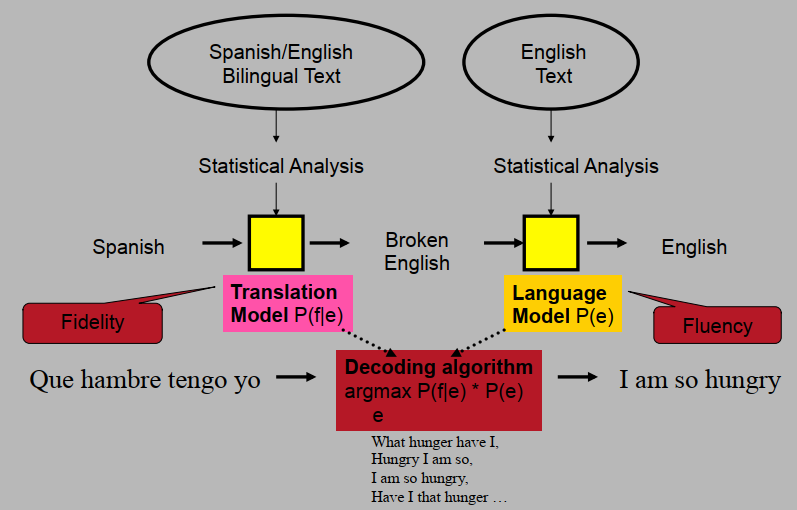
\includegraphics[width=10cm]{figures/smt.png}
    \caption{Example of Spanish-English SMT system.}
\end{figure}

The translation model in the first step needs to know which words to align in a source-target sentence pair. More in the next section.

\section{Word alignments}

Word alignment between two texts is the NLP task of identifying translation relationships among the words in a parallel text, resulting in a graph between the two sides of the texts, with an arc between two words if they are translations of one another. See the following example:

\begin{figure}[!ht]
    \centering
    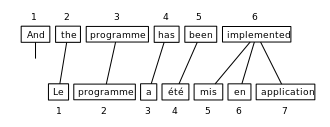
\includegraphics[width=10cm]{figures/word_align.png}
    \caption{Word alignments between an English and French sentence.}
\end{figure}

Alternatively, the alignments can also be displayed in a matrix:

\begin{figure}[!ht]
    \centering
    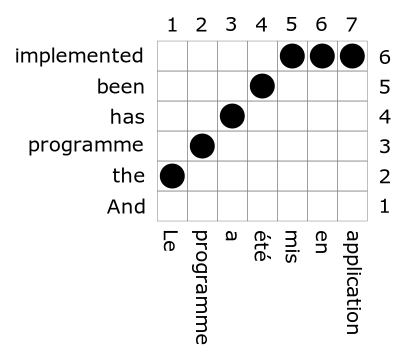
\includegraphics[width=8cm]{figures/word_align_matrix.png}
    \caption{Word alignments between an English and French sentence in matrix form.}
\end{figure}

In this example, the alignments aren't 1-on-1. Some words have a direct alignment, such as \emph{the}-\emph{le}, \emph{programme}-\emph{programme} and so on, but some words don't have an alignment (\emph{And}), and some have multiple alignments, in this case one-to-many: \emph{inmplemented}-\emph{mis en application}. There can also be many-to-one and many-to-many alignments.

Word alignment is an important task for most methods of statistical machine translation, since the parameters of these methods are usually estimated by observing word-aligned texts~\cite{brown1993mathematics}, and automatic word alignment is typically done by choosing that alignment which best fits a statistical machine translation model. A popular algorithm to find word alignments is the \emph{expectation-maximization algorithm}~\cite{och1999improved}

This approach is an example of unsupervised learning, meaning that the system has no knowledge of the kind of output desired, but tries to find values for the unobserved model and alignments which best explain the observed parallel text. In some cases, a small number of manually aligned sentences, in a way to explore supervised learning.~\cite{varga2007parallel} These models are usually able to more easily take advantage of combining many features within the data, such as context, syntactic structure, part-of-speech or translation lexicon information, which are difficult to integrate into the unsupervised models generally used.

For training, historically IBM models have been used.~\cite{koehn2009statistical} These models are used in statistical machine translation to train a) a translation model, and b) an alignment model. They make use of the expectation-maximization algorithm explained above: in the expectation step, the translation probabilities within each sentence are computed; in the maximization step, these probabilities are accumulated to global translation probabilities.

\subsection{Fastalign algorithm}

Fastalign algorithm~\cite{dyer-etal-2013-simple}

is a simple log-linear reparametrization of IBM Model 2 that overcomes problems from both Model 1 and Model 2. Training this model is consistently ten times faster than Model 4.

An open-source implementation of the alignment model described in this paper is available in \href{http://github.com/clab/fast align}{Github}.

Fastalign is a variation of the lexical translation. Lexican translation works as follows: given a source sentence \emph{f} with length \emph{n}, first generate the length of the target sentence \emph{m}, where the target sentence is \emph{e}. Then generate an alignment vector of length \emph{m} that indicates which source word (or null token) each target word will be a translation of. Lastly, generate the \emph{m} output words, where each word in \emph{e} depends only on the word in \emph{f} it's aligned with.

Fastalign's modification is that the distribution over alignments is parametrized by a null alignment probability and a precision parameter, which controls how strongly the model favors alignment points close to the diagonal (if we use the word alignment matrix like in the example above).

The paper~\cite{dyer-etal-2013-simple} has more detailed information on training, inference and results.

\subsection{Eflomal algorithm}

https://github.com/robertostling/eflomal
https://content.sciendo.com/view/journals/pralin/106/1/article-p125.xml
% Template for a Thesis
%
% 5-methodology.tex
%
% Methodology

\chapter{Methodology}\label{sec:methodology}

Theoretical idea: what I want to do, how, algorithmic/mathematical

This chapter explains the technical content of this thesis in broad strokes, the methodology used and the general idea of the methods employed. For a more in-depth analysis, refer to the next chapter.

This thesis, first of all, aims to replicate the results of BPE and BPE dropout.

\section{Replication of BPE results}

Using Sennrich et al.'s~\cite{sennrich2015neural} \href{code on Github}{https://github.com/rsennrich/subword-nmt/}, the first goal was to check the gold standard's alignment scores. For that, these steps were undertaken:

\begin{enumerate}
	\item Write learn BPE from corpus algorithm
	\item Write apply BPE to corpus algorithm
	\item Write extract alignment script
	\item Write calculate alignment scores script
\end{enumerate}

The actual code for each step can be found in the next section, Development.

The corpus is a 10k sentence English-German corpus, containing an index number for each sentence. As an excerpt of the corpora:

\begin{quote}
	English\\
	21	The Committee on Transport and Tourism has adopted four amendments for the second reading .\\
	22	They will certainly enhance the feeling of the right of movement by EU citizens and they will also certainly benefit disabled drivers .\\
	23	The initial Commission proposal was adopted unamended by Parliament on first reading .\\\\
	German\\
	21	Der Transportausschuß hat für die zweite Lesung vier Änderungsanträge beschlossen .\\
	22	Sie werden bei den EU-Bürgern gewiß das Gefühl für das Recht auf Freizügigkeit stärken , und sie werden gewiß auch behinderten Fahrern Vorteile bringen .\\
	23	Der ursprüngliche Vorschlag der Kommission wurde vom Parlament in erster Lesung ohne Änderungen verabschiedet .
\end{quote}

\subsection{Learn BPE algorithm}

Sennrich's repository's code has some additional parameters that weren't relevant for a minimal implementation of the BPE algorithm, so the script was adapted. These are the steps for a minimal learn BPE algorithm:

\begin{enumerate}
	\item Read corpus into tokens, parse index.
	\item Count pair frequencies.
	\item Start loop from 1 until desired vocabulary size. In our case, 10k merges.
	\begin{enumerate}
		\item Get most frequent pair.
		\item Append most frequent pair to vocabulary.
		\item Merge pair in corpus.
		\item Count pair frequencies in corpus.
	\end{enumerate}
	\item Write vocabulary to a file.
\end{enumerate}

This step of the pipeline only has to be done once for each corpus, afterwards the vocabulary can be used in different ways. But this minimal algorithm, since it has to count all the pairs in the whole corpus in each iteration, takes a long time. An optimization came after this.

\subsection{Apply BPE algorithm}

Once the vocabulary has been learnt, it can be applied to a corpus. In this case, we use the same corpus for training and for applying. To generate different output files, different num\_merges are declared. For example, for 500 merges, only the first 500 merges of the vocabulary are considered, and there aren't many recognizable BPE units in the corpus. For bigger merge values, more and more subword units get merged. In this thesis, the following merges have been considered: [100, 200, 500, 1000, 2000, 4000, 6000, 8000]. These are the steps for this part:

\begin{enumerate}
	\item Load data, corpus and BPE vocabulary.
	\item Start loop for all numbers of merges.
	\begin{enumerate}
		\item Start loop from 1 until desired amount of merges.
		\begin{enumerate}
			\item Merge corpus for current most frequent pair.
		\end{enumerate}
		\item Write to output.bpe file.
	\end{enumerate}
\end{enumerate}

For example, this is what the excerpt from the corpora above look like after 100 merges:

\begin{quote}
	English\\
	\_the \_Comm it t e e \_on \_T ran s p ort \_and \_T ouris m \_has \_a d o p t ed \_f our \_a m end ment s \_for \_the \_sec ond \_re a d ing \_.\\
	\_the y \_w ill \_cer t a in ly \_en h an ce \_the \_f e e ling \_of \_the \_ri g h t \_of \_m o ve ment \_b y \_E U \_citi z en s \_and \_the y \_w ill \_al s o \_cer t a in ly \_ben e f it \_d is a bled \_d ri ver s \_.\\
	\_the \_in iti al \_Commission \_pro p o s al \_w as \_a d o p t ed \_u n a m end ed \_b y \_P ar li a ment \_on \_f ir st \_re a d ing \_.\\\\
	German\\
	\_der \_T rans p or t a ussch u ß \_h at \_für \_die \_z w eite \_L es ung \_v ier \_Ä nder ung s ant r ä ge \_besch l o ss en \_.\\
	\_s ie \_wer den \_bei \_den \_E U - B ür ger n \_ge w i ß \_das \_G e f ü h l \_für \_das \_Re ch t \_auf \_F r ei z ü g i g k eit \_st ä r k en \_, \_und \_s ie \_wer den \_ge w i ß \_au ch \_beh inder ten \_F a hr er n \_V or tei l e \_b r ingen \_.\\
	\_der \_ur s p r ü ng lich e \_V or sch la g \_der \_Ko mm iss ion \_w ur de \_v o m \_P ar la ment \_in \_er ster \_L es ung \_o h n e \_Ä nder ungen \_vera b sch ie det \_.
\end{quote}

Only the 100 most common units in the language have been merged, so in English we can see the merge of \emph{\_the}, \emph{\_and}, \emph{ment}, and other very common words and affix/suffixes. As for German, we can see very common words being merged such as \emph{\_die}, \emph{\_das}, \emph{\_bei} and so on. When we do 4000 merges:

\begin{quote}
	English\\
	\_the \_Committee \_on \_Transport \_and \_Tourism \_has \_adopted \_four \_amendments \_for \_the \_second \_reading \_.\\
	\_they \_will \_certainly \_enhance \_the \_feeling \_of \_the \_right \_of \_movement \_by \_EU \_citizens \_and \_they \_will \_also \_certainly \_benefit \_dis abled \_drivers \_.\\
	\_the \_initial \_Commission \_proposal \_was \_adopted \_un amended \_by \_Parliament \_on \_first \_reading \_.\\\\
	German\\
	\_der \_T ransp ortausschuß \_hat \_für \_die \_zweite \_Lesung \_vier \_Änderungsanträge \_beschlossen \_.\\
	\_sie \_werden \_bei \_den \_EU-B ür gern \_gew iß \_das \_Ge fü hl \_für \_das \_Recht \_auf \_Freizügigkeit \_stärken \_, \_und \_sie \_werden \_gew iß \_auch \_behinderten \_Fahrern \_Vorteile \_bringen \_.\\
	\_der \_ursprüngliche \_Vorschlag \_der \_Kommission \_wurde \_vom \_Parlament \_in \_erster \_Lesung \_ohne \_Änderungen \_verabschiedet \_.
\end{quote}

Most words are merged, except \emph{\_dis abled} in English, and \emph{\_T ransp ortausschuß} in German for instance.

\subsection{Extract alignments}

Write extract alignment script to align files from 2 different languages using fastalign/eflomal

To evaluate if the BPE units are good, bilingual corpora are aligned, and then compared against a gold standard. On the first step, alignment, two algorithms have been used, fastalign and eflomal. The software installation guides can be found in the development section.

These algorithms take English text and German as input and create an alignment file as output. For the example above:

\begin{quote}
	English sentence: The Committee on Transport and Tourism has adopted four amendments for the second reading .\\
	German sentence: Der Transportausschuß hat für die zweite Lesung vier Änderungsanträge beschlossen .\\
	Alignment: 0-0 1-1 2-1 3-1 4-1 5-1 6-2 7-9 8-7 9-8 10-3 11-4 12-5 13-6 14-10\\

	English sentence: The initial Commission proposal was adopted unamended by Parliament on first reading .\\
	German sentence: Der ursprüngliche Vorschlag der Kommission wurde vom Parlament in erster Lesung ohne Änderungen verabschiedet .\\
	Alignment: 0-0 1-1 2-4 3-2 3-3 4-5 5-13 6-11 6-12 7-6 8-7 9-8 10-9 11-10 12-14
\end{quote}

Many words have one-to-one alignment, such as \emph{four}-\emph{vier}, \emph{adopted}-\emph{verabschiedet} and many others. Some others have many-to-one alignments, such as \emph{Committee on Transport and Tourism}-\emph{Transportausschuß} and one-to-many alignments such as \emph{unamended}-\emph{ohne Änderungen}.

In our case however, the input files aren't composed by words, but rather by subwords. And the alignments are done among subwords. As with the example with 4000 merges:

\begin{quote}
	English sentence: \_the \_Committee \_on \_Transport \_and \_Tourism \_has \_adopted \_four \_amendments \_for \_the \_second \_reading \_.\\
	German sentence: \_der \_T ransp ortausschuß \_hat \_für \_die \_zweite \_Lesung \_vier \_Änderungsanträge \_beschlossen \_.\\
	Alignment: 0-0 1-1 2-1 3-1 4-1 5-1 1-2 2-2 3-2 4-2 5-2 1-3 2-3 3-3 4-3 5-3 6-4 7-11 8-9 9-10 10-5 11-6 12-7 13-8 14-12
\end{quote}

Since the German word \emph{Transportausschuß} is divided into three, namely \emph{T ransp ortausschuß}, the many-to-one alignment from the previous case is now a many-to-many alignment. Now there are subword alignments as opposed to word alignments. The number of alignment has grown from last example.

Because the gold standard against which the system is being evaluated consists of word alignments, it's necesssary to map subword alignments into word alignments.

This script takes English and German corpora and the alignment file as inputs, and outputs a word alignment file.

\begin{quote}
	English sentence: \_the \_Committee \_on \_Transport \_and \_Tourism \_has \_adopted \_four \_amendments \_for \_the \_second \_reading \_.\\
	German sentence: \_der \_T ransp ortausschuß \_hat \_für \_die \_zweite \_Lesung \_vier \_Änderungsanträge \_beschlossen \_.\\
	Subword alignment: 0-0 1-1 2-1 3-1 4-1 5-1 1-2 2-2 3-2 4-2 5-2 1-3 2-3 3-3 4-3 5-3 6-4 7-11 8-9 9-10 10-5 11-6 12-7 13-8 14-12\\
	Output word alignment: 0-0 1-1 2-1 3-1 4-1 5-1 6-2 7-9 8-7 9-8 10-3 11-4 12-5 13-6 14-10
\end{quote}

The challenge here lies in the fact that if the BPEs are of good quality, the alignment algorithm will align subword items correctly, and therefore in the subword-to-word mapping, the word alignments will be correct.

\begin{quote}
	a\\
\end{quote}

\begin{enumerate}
	\item 
\end{enumerate}
% Template for a Thesis
%
% 6-development.tex
%
% Development

\chapter{Development}\label{sec:development}

This chapter talks more deeply about the code and algorithms previously explained in the Methodology section.~\ref{sec:methodology}

\section{Coding practices}

The parameters for the pipeline, such as num\_symbols, dropout, file paths, etc. have been written in \emph{settings.py}.

\begin{python}
# global variables
import os
from os.path import join
import sys

word_sep = u'\u2581'
source, target = 'eng', 'deu'

num_all_symbols = 20000
all_symbols = [100, 200, 500, 1000, 2000, 4000, 6000, 8000]

rootdir = os.getcwd()
if rootdir.split(os.sep)[-1] == 'src':
    rootdir = os.sep.join(rootdir.split(os.sep)[:-1])

datadir = join(rootdir, 'data')
inputdir = join(datadir, 'input')
bpedir = join(datadir, 'dropout_bpe' if dropout > 0 else 'normal_bpe')
baselinedir = join(rootdir, 'reports', 'scores_normal_bpe')
scoredir = join(rootdir, 'reports', 'scores_' + ('dropout_bpe' if dropout > 0 else 'normal_bpe'))
goldpath = join(inputdir, 'eng_deu.gold')
inputpath = {source: join(inputdir, source+'_with_10k.txt'),
            target: join(inputdir, target+'_with_10k.txt')}

fastalign_path = join(rootdir, "tools/fast_align/build/fast_align")
atools_path = join(rootdir, "tools/fast_align/build/atools")
    
\end{python}

\section{Replication of BPE results}

\begin{enumerate}
    \item Write learn BPE from corpus algorithm
    \item Write apply BPE to corpus algorithm
    \item Write extract alignment script
    \item Write calculate alignment scores script
\end{enumerate}

\subsection{Learn BPE algorithm}

\begin{python}
#!/usr/bin/env python

import os
import re
import sys
import codecs
from tqdm import tqdm
from os.path import join
from collections import defaultdict, Counter

# import global variables from settings.py
sys.path.insert(1, os.path.join(sys.path[0], '..'))
from settings import *

def read_corpus(corpus: list) -> list:
  """
  Read corpus, strip index and new line characters.
  In space mode, each word has a word_sep symbol at the beginning to signal it's the beginning of the word.
  example:
  tokens = [
      '\_w e \_d o \_n o t \_b e l i e v e 
      \_t h a t \_w e \_s h o u l d 
      \_c h e r r y - p i c k \_.',
      ...
  ]
  """

  tokens = []
  for line in corpus:
    line = line.split('\t')[1].strip('\r\n ')
    line = line.split()
    line[0] = str.lower(line[0])

    # add word_sep to each beginning of word and join by space
    tokens.append(' '.join([word_sep + ' '.join(word) for word in line]))

  return tokens

def get_stats(tokens: list) -> Counter:
  """
  Count frequency of all bigrams and the frequency per index.
  pairs = {
    ('s', 'h'): 5,
    ('h', 'e'): 6
  }
  The last token '.' or word_sep. isn't merged with anything.
  """

  pairs = Counter()
  for i, sent in enumerate(tokens):
    # get stats for each word independently, 
    # no bigrams between different words
    for word in sent[1:].split(' '+word_sep):
      symbols = symbols.split()
      for j in range(len(symbols) - 1):
        pairs[symbols[j], symbols[j + 1]] += 1

  return pairs


def merge_token(corpus, most_frequent):
  str_corpus = '\n'.join(corpus)
  str_corpus = str_corpus.replace(' '.join(most_frequent), ''.join(most_frequent))
  return str_corpus.split('\n')


def learn_bpe(argsinput, bpe_model):
  """
  Learn BPE operations from vocabulary.
  Steps:
  1. split corpus into characters, count frequency
  2. count bigrams in corpus
  3. merge most frequent symbols
  4. Update bigrams in corpus 
  """

  corpus = read_corpus(argsinput)

  most_frequent_merges = []
  for i in range(num_all_symbols):

    pairs = get_stats(corpus)

      try:
        most_frequent = pairs.most_common(1)[0][0]
      except:
        # pairs is empty
        break

      most_frequent_merges.append(most_frequent)
      corpus = merge_token(corpus, most_frequent)

  return most_frequent_merges


def write_bpe(lang, most_freq_merges):

  bpe_file = codecs.open(join(datadir, lang+'.model'), 'w', encoding='utf-8')
  bpe_file.write(f"{lang} {len(most_freq_merges)}\n")
  bpe_file.write('\n'.join(' '.join(item) for item in most_freq_merges))
  return

if __name__ == '__main__':

  for lang in [source, target]:

    argsinput = codecs.open(inputpath[lang], encoding='utf-8')
    bpe_model = codecs.open(join(datadir, lang+'.model'), 'w', encoding='utf-8')
    most_freq_merges = learn_bpe(argsinput, bpe_model)
    write_bpe(lang, most_freq_merges)
\end{python}

\subsection{Apply BPE algorithm}

\begin{python}
# apply_bpe.py

import os
from os.path import join
import sys
import codecs
import random
from tqdm import tqdm

# import global variables from settings.py
sys.path.insert(1, os.path.join(sys.path[0], '..'))
from settings import *
from learn_bpe import read_bpe_model, read_corpus

def load_data():

  os.chdir(datadir)
  langs = [source, target]
  bpe_models = []
  corpora = []
  for lang in langs:

    argsinput = codecs.open(inputpath[lang], encoding='utf-8')
    corpora.append(read_corpus(argsinput))

    bpe_model, _ = read_bpe_model(lang)
    if not bpe_model:
      print(f"No model found for lang={lang}")

    bpe_model = [tuple(item.strip('\r\n ').split(' ')) for (n, item) in enumerate(bpe_model)]
    bpe_models.append(bpe_model[1:])

  return langs, bpe_models, corpora

def write_bpe(lang, num_symbols, merged_corpus):
  outputpath = join(bpedir, 'segmentations', f"{lang}_{num_symbols}.bpe")
  argsoutput = codecs.open(outputpath, 'w', encoding='utf-8')
  argsoutput.write(merged_corpus)
  return

def apply_bpe(langs, bpe_models, corpora):
    
  for lang, bpe_model, corpus in zip(langs, bpe_models, corpora):

    bpe_model = bpe_model[:max(all_symbols)]
    all_symbols_copy = all_symbols.copy()

    str_corpus = '\n'.join(corpus)
    for j, bigram in enumerate(bpe_model):

      str_corpus = str_corpus.replace(' '.join(bigram), ''.join(bigram))

      if j + 1 == all_symbols_copy[0]:
        write_bpe(lang, all_symbols_copy.pop(0), str_corpus)
  return

if __name__ == "__main__":

  os.makedirs(join(bpedir, 'segmentations'), exist_ok=True)
  langs, bpe_models, corpora = load_data()
  apply_bpe()
\end{python}

\subsection{Extract alignments}

In the next step, the extract alignments script takes two files as input: English BPE file, German BPE file, and outputs an alignment file, with the extension .wgdfa.

First of all, it's necessary to iterate through the different merge types that have been done before. There are BPE files with 100 merges, 200, 500, etc for both languages. At each iteration, a different alignment file is created.

Alignment algorithms work on parallel data, that is, they expect text in the following format:

\begin{quote}
  Hello from England ||| Hallo aus Deutschland
\end{quote}

Since the BPE files don't have this format, first of all the function \emph{create\_parallel\_text} creates a \emph{.txt} file in the appropriate format. Afterwards, both \emph{fastalign} and \emph{eflomal} generate forward and reverse alignments. This is handled by the \emph{create\_fwd\_rev\_files} function, which creates \emph{.fwd} and \emph{.rev} files. Afterwards, given these \emph{.fwd} and \emph{.rev} files, the alignment algorithm creates a type of union between these two, called \emph{grow-diag-final-and}, with the extension \emph{.gdfa}. This is handled by the \emph{create\_gdfa\_file} function.

As explained in the \textit{Extract alignment} subsection in the Methodology chapter~\ref{subsec:extractalign}, the script up until now has only aligned BPE units. Those alignments need to be transformed into word alignments. The function \emph{load\_and\_map\_segmentations} loads the BPE files and maps each BPE unit to its corresponding word. For an example, see the comments on the function. This is an auxiliary function in order to map the alignments later. Afterwards, by calling \emph{bpe\_word\_align}, the mapping from subword alignments to word alignments is made. Lastly, the new alignments are saved in a file with the extension \emph{.wgdfa}.

The alignment algorithm is run for two types of files. Firstly, for the corpus itself, the fastalign/eflomal algorithm is run to align the corpus, which will serve as baseline to check how good the BPE merges are. And then, the fastalign/eflomal algorithm is run for the BPE files themselves.

\begin{python}
# extract_alignments.py

from os.path import join
import os
import sys
import codecs

# import global variables from settings.py
sys.path.insert(1, os.path.join(sys.path[0], '..'))
from settings import *
from subword_word import *

def create_parallel_text(sourcepath, targetpath, outpath):

  fa_file = codecs.open(outpath + '.txt', "w", "utf-8")
  fsrc = codecs.open(sourcepath, "r", "utf-8")
  ftrg = codecs.open(targetpath, "r", "utf-8")

  for sl, tl in zip(fsrc, ftrg):
    sl = sl.strip().split("\t")[-1]
    tl = tl.strip().split("\t")[-1]
    fa_file.write(f"{sl} ||| {tl}\n")
  fa_file.close()
  return

def create_fwd_rev_files(outpath):
  if mode == "fastalign":
    os.system(f"{fastalign_path} -i {outpath}.txt -v -d -o > {outpath}.fwd")
    os.system(f"{fastalign_path} -i {outpath}.txt -v -d -o -r > {outpath}.rev")
  elif mode == "eflomal":
    os.system(f"cd {eflomal_path}; python align.py -i {outpath}.txt --model 3 -f {outpath}.fwd -r {outpath}.rev")
  return

def create_gdfa_file(outpath):
  # create gdfa file from .fwd and .rev
  os.system(f"{atools_path} -i {outpath}.fwd -j {outpath}.rev -c grow-diag-final-and > {outpath}_unnum.gdfa")

  # parse _unnum.gdfa to .gdfa with "\t" separator
  with codecs.open(f"{outpath}_unnum.gdfa", "r", "utf-8") as fi, codecs.open(f"{outpath}.gdfa", "w", "utf-8") as fo:
    for i, line in enumerate(fi):
      fo.write(f"{i}\t{line.strip()}\n")

  # delete unnecessary files
  os.system(f"rm {outpath}_unnum.gdfa; rm {outpath}.fwd; rm {outpath}.rev; rm {outpath}.txt")
  return

def load_and_map_segmentations(num_symbols):

    '''
    Given a .bpe file composed of the corpus made of subword units such as
    corpus_eng =  [
        '_We _do _no t _be li eve _.',
        '_Thi s _is _a _sent ence _.',
        ...
    ]
    Output: dictionary of each language and 
    a list of indexes pointing to which word each element (_do) belongs to
    bpes = {
        'eng':
        [
            [0, 1, 2, 2, 3, 3, 3, 4],
            [0, 0, 1, 2, 3, 4, 5],
            ...
        ],
        'deu':
        [
            ...
        ],
    } 
    '''

    bpes = {}
    for lang in [source, target]:

        bpes[lang] = []
        corpus = codecs.open(lang+'_'+str(num_symbols)+'.bpe', encoding='utf-8')
        for sent in corpus:
          mapping = [0]
          i = 0
          for subw in sent.split()[1:]:
              if subw[0] == word_sep:
                i += 1
              mapping.append(i)
          bpes[lang].append(mapping)
    return bpes

def bpe_word_align(bpes, bpe_aligns):
    '''
    Input: dictionary of bpes obtained as output of map_subword_to_word()
    Output: list of word alignments and their indexes
        "
            0   0-0 0-1 1-1 1-2 3-1 2-4 \n
            1   0-0 1-0 1-1 2-1 \n
            ...
        "
    '''
    all_word_aligns = ''
    for i, (sent1, sent2, bpe_al) in enumerate(zip(bpes[source], bpes[target], bpe_aligns)):
        word_aligns = set()
        # iterate each alignment
        for al in bpe_al.split('\t')[1].split():
            firstal, secondal = al.split('-')
            new_al = str(sent1[int(firstal)]) + '-' + str(sent2[int(secondal)])
            word_aligns.add(new_al)
        all_word_aligns += str(i) + "\t" + ' '.join(word_aligns) + "\n"
    return all_word_aligns

def extract_alignments(input_mode=False):

  for num_symbols in all_symbols:

    if input_mode:
      print("Alignments for input files")
      sourcepath = inputpath[source]
      targetpath = inputpath[target]
      outpath = join(bpedir, mode, "input")
    else:
      print(f"Alignments for {num_symbols} symbols")
      sourcepath = join(bpedir, 'segmentations', f"{source}_{num_symbols}.bpe")
      targetpath = join(bpedir, 'segmentations', f"{target}_{num_symbols}.bpe")
      outpath = join(bpedir, mode, str(num_symbols))

    create_parallel_text(sourcepath, targetpath, outpath)
    create_fwd_rev_files(outpath)
    create_gdfa_file(outpath)

    # map alignment from subword to word
    bpes = load_and_map_segmentations(num_symbols)

    argsalign = codecs.open(o+'.gdfa', encoding='utf-8')
    all_word_aligns = bpe_word_align(bpes, argsalign)
    os.system(f"rm {outpath}.gdfa")

    argsoutput = codecs.open(outpath+'.wgdfa', 'w', encoding='utf-8')
    argsoutput.write(all_word_aligns)

  return

if __name__ == "__main__":

  os.makedirs(join(bpedir, mode), exist_ok=True)
  if not os.path.isfile(join(bpedir, mode, 'input.wgdfa')):
    extract_alignments(input_mode=True)

  extract_alignments()
\end{python}

\subsection{Calculate alignment scores}

The last script calculates the alignment scores. These are the steps of the script:

\begin{enumerate}
  \item Load gold dataset
  \item Calculate precision, recall, F1 score and AER metrics
  \item Plot and save into \emph{.png} and \emph{.csv}
\end{enumerate}

\begin{python}
# calc_align_scores.py

import os
from os.path import join
import sys
import glob
import random
import collections
import pandas as pd
import matplotlib.pyplot as plt
import seaborn as sns

# import global variables from settings.py
sys.path.insert(1, os.path.join(sys.path[0], '..'))
from settings import *

def load_gold(g_path):

  gold_f = open(g_path, "r")
  pros = {}
  surs = {}
  all_count = 0.
  surs_count = 0.

  for line in gold_f:
    line = line.strip().split("\t")
    line[1] = line[1].split()

    pros[line[0]] = set()
    surs[line[0]] = set()

    for al in line[1]:
      pros[line[0]].add(al.replace('p', '-'))
      if 'p' not in al:
        surs[line[0]].add(al)

    all_count += len(pros[line[0]])
    surs_count += len(surs[line[0]])

  return pros, surs, surs_count

def calc_score(input_path, probs, surs, surs_count):

  total_hit = 0.
  p_hit = 0.
  s_hit = 0.
  target_f = open(input_path, "r")

  for line in target_f:
    line = line.strip().split("\t")

    if line[0] not in probs: continue
    if len(line) < 2: continue

    line[1] = line[1].split()
    for pair in line[1]:
      if pair in probs[line[0]]:
        p_hit += 1
      if pair in surs[line[0]]:
        s_hit += 1

      total_hit += 1

  target_f.close()

  y_prec = round(p_hit / max(total_hit, 1.), 3)
  y_rec = round(s_hit / max(surs_count, 1.), 3)
  y_f1 = round(2. * y_prec * y_rec / max((y_prec + y_rec), 0.01), 3)
  aer = round(1 - (s_hit + p_hit) / (total_hit + surs_count), 3)

  return y_prec, y_rec, y_f1, aer

def get_baseline_score(probs, surs, surs_count):

  alfile = join(bpedir, mode, 'input.wgdfa')

  scores = []
  score = [0]
  score.extend(list(calc_score(alfile, probs, surs, surs_count)))
  scores.append(score)
  baseline_df = pd.DataFrame(scores, columns=['num_symbols', 'prec', 'rec', 'f1', 'AER']).round(decimals=3)
  return baseline_df

def calc_align_scores(probs, surs, surs_count):

  scores = []
  for num_symbols in all_symbols:
    alfile = join(bpedir, mode, f"{num_symbols}.wgdfa")
    
    score = [int(num_symbols)]
    score.extend(list(calc_score(alfile, probs, surs, surs_count)))
    scores.append(score)

  df = pd.DataFrame(scores, columns=['num_symbols', 'prec', 'rec', 'f1', 'AER']).round(decimals=3)
  return df


def plot_scores(df, baseline_df, scoredir):

  # Use plot styling from seaborn.
  sns.set(style='darkgrid')

  # Increase the plot size and font size.
  sns.set(font_scale=1.5)
  plt.rcParams["figure.figsize"] = (12, 6)

  plt.clf()
  ax = plt.gca() # gca stands for 'get current axis'

  colors = ['magenta', 'tab:blue', 'tab:green', 'tab:red']

  df = df.sort_values('num_symbols')
  columns = list(df)
  for column, color in zip(columns[1:], colors):
    df.plot(kind='line', x=columns[0], y=column, color=color, ax=ax)

  for baseline_results, color in zip(list(baseline_df.iloc[0][1:]), colors):
    plt.axhline(y=baseline_results, color=color, linestyle='dashed')

  plt.savefig(join(scoredir+'.png'))
  return


if __name__ == "__main__":
  '''
  Calculate alignment quality scores based on the gold standard.
  The output contains Precision, Recall, F1, and AER.
  '''

  probs, surs, surs_count = load_gold(goldpath)
  baseline_df = get_baseline_score(probs, surs, surs_count)
  df = calc_align_scores(probs, surs, surs_count, baseline_df)

  scorename = join(scoredir, 'scores')
  print(f"Scores saved into {scorename}")
  df.to_csv(scorename+'.csv', index=False)
  plot_scores(df, baseline_df, scorename)

\end{python}

\section{Replication of BPE dropout}

The previous section has laid the backbone of the algorithms. In this and the following sections, some modifications are introduced. For the sake of simplicity, the code snippets that follow only include the new changes, or the functions from the last section with new modifications. The functions that remain unaltered aren't shown.

Two new parameters come into play in the pipeline, namely \textbf{dropout} rate and \textbf{dropout\_samples}, that is, how many samples of the dropout system are considered. These values are saved into \emph{settings.py}

\begin{python}
# settings.py

dropout = 0.1
dropout_samples = 10
\end{python}

\subsection{Apply BPE to corpus with dropout}

The first modifications are in \emph{apply\_bpe.py}, where we skip some merges, and repeat the process 10 times. The function \emph{apply\_bpe} includes two new lines where a random number between 0 and 1 is generated. If this number is smaller than the \emph{dropout} rate saved in \emph{settings.py}, then that merge isn't considered and the loop skips it. Additionally, in the main function, the function \emph{apply\_bpe} is called \emph{dropout\_samples} times. To save the files accordingly, a new variable is introduced, namely \emph{i}, that does nothing in the case where dropout=0, but when repeating the process, for instance if lang=eng, num\_symbols=2000, and first iteration of dropout, that is, i=0, the files are saved as \emph{eng\_2000\_0.bpe} instead.

\begin{python}
# apply_bpe.py
import random

def write_bpe(lang, num_symbols, merged_corpus, i=-1):

  outputpath = join(bpedir, 'segmentations', f"{lang}_{num_symbols}{f'_{i}' if i != -1 else ''}.bpe")
  argsoutput = codecs.open(outputpath, 'w', encoding='utf-8')
  argsoutput.write(merged_corpus)
  return

def apply_bpe(langs, bpe_models, corpora, i=-1):
    
  for lang, bpe_model, corpus in zip(langs, bpe_models, corpora):

    bpe_model = bpe_model[:max(all_symbols)]
    all_symbols_copy = all_symbols.copy()
    str_corpus = '\n'.join(corpus)

    for j, bigram in enumerate(bpe_model):

        if random.uniform(0, 1) < dropout:
            continue

      str_corpus = str_corpus.replace(' '.join(bigram), ''.join(bigram))

      if j + 1 == all_symbols_copy[0]:
        write_bpe(lang, all_symbols_copy.pop(0), str_corpus, i)
  return

if __name__ == "__main__":

  langs, bpe_models, corpora = load_data()

  if dropout > 0:
    for i in range(dropout_samples):
      apply_bpe(i)
  else:
      apply_bpe()
\end{python}

\subsection{Extract alignments with dropout}

The only change here is that the \emph{extract\_alignment} function is called \emph{dropout\_samples} times, which changes the function to write the alignments in the new format, namely, changing the variables \emph{sourcepath} and \emph{targetpath}. The rest, the alignment algorithm, remains unchanged.

\begin{python}
# extract_alignments.py

def extract_alignments(i=-1, input_mode=False):

  for num_symbols in all_symbols:

    if input_mode:
      print("Alignments for input files")
      sourcepath = inputpath[source]
      targetpath = inputpath[target]
      outpath = join(bpedir, mode, "input")
    else:
      print(f"Alignments for {num_symbols} symbols")
      sourcepath = join(bpedir, 'segmentations', f"{source}_{num_symbols}_{'_'+str(i) if dropout else ''}.bpe")
      targetpath = join(bpedir, 'segmentations', f"{target}_{num_symbols}_{'_'+str(i) if dropout else ''}.bpe")
      outpath = join(bpedir, mode, str(num_symbols))

    create_parallel_text(sourcepath, targetpath, outpath)
    create_fwd_rev_files(outpath)
    create_gdfa_file(outpath)

    # map alignment from subword to word
    bpes = load_and_map_segmentations(num_symbols)

    argsalign = codecs.open(o+'.gdfa', encoding='utf-8')
    all_word_aligns = bpe_word_align(bpes, argsalign)
    os.system(f"rm {outpath}.gdfa")

    argsoutput = codecs.open(outpath+'.wgdfa', 'w', encoding='utf-8')
    argsoutput.write(all_word_aligns)

  return

if __name__ == "__main__":

  os.makedirs(join(bpedir, mode), exist_ok=True)
  if not os.path.isfile(join(bpedir, mode, 'input.wgdfa')):
    extract_alignments(input_mode=True)

  if dropout > 0:
    for i in range(dropout_samples):
      extract_alignments(i)
  else:
    extract_alignments()
\end{python}

\subsection{Calculate alignment scores with dropout}

As explained in the Methodology section~\ref{sec:replbpedrop}, variants of union, intersection and threshold are created. This is introduced with a new algorithm, namely \emph{merge\_dropout.py}. First of all, the function \emph{merge\_dropout\_alignments} opens all alignment files and creates a dictionary data structure with the union, intersection and threshold alignment files and saves them into \emph{X\_union.wgdfa}, \emph{X\_inter.wgdfa}, \emph{X\_thres.wgdfa} respectively. Afterwards, the function \emph{calc\_score\_merges} opens these files and calculates the score, much in the way as the \emph{calc\_align\_score} algorithm from the previous section.

\begin{python}
# merge_dropout.py
import os
from os.path import join
import sys
import codecs
import pandas as pd
from tqdm import tqdm
from collections import Counter

# import global variables from settings.py
sys.path.insert(1, os.path.join(sys.path[0], '..'))
from settings import *
from calc_align_score import *

def merge_dropout_alignments():
  union_merge, inter_merge, thres_merge = {}, {}, {}

  os.chdir(join(bpedir, mode))
  for num_symbols in tqdm(all_symbols, desc=f"merge_dropout: dropout={dropout}, union, inter, thres"):
    union_merge[num_symbols], inter_merge[num_symbols], thres_merge[num_symbols] = [], [], []

    for i in range(dropout_sampless):

      for j, line in enumerate(open(f'{num_symbols}_{i}.wgdfa', 'r').readlines()):
        al = frozenset(line.strip().split("\t")[1].split())

        # at the first iteration, just append the alignment
        if i == 0:
          union_merge[num_symbols].append(al)
          inter_merge[num_symbols].append(al)
          thres_merge[num_symbols].append(Counter(al))
          continue
        
        # do union, intersection or frequency addition
        union_merge[num_symbols][j] |= al
        inter_merge[num_symbols][j] &= al
        thres_merge[num_symbols][j] += Counter(al)

    # write to output
    unionfile = codecs.open(f'{num_symbols}_union.wgdfa', 'w')
    interfile = codecs.open(f'{num_symbols}_inter.wgdfa', 'w')
    thresfiles = {merge_t: codecs.open(f'{num_symbols}_thres_{merge_t}.wgdfa', 'w') for merge_t in merge_threshold}

    for i in range(len(union_merge[num_symbols])):
      unionfile.write(f"{i}\t{' '.join(union_merge[num_symbols][i])}\n")
      interfile.write(f"{i}\t{' '.join(inter_merge[num_symbols][i])}\n")

      # get alignments more common than the merge_threshold %
      for merge_t in merge_threshold:
        common_aligns = [k for k in thres_merge[num_symbols][i] 
                        if thres_merge[num_symbols][i][k] > merge_t * dropout_samples]
        thresfiles[merge_t].write(f"{i}\t{' '.join(common_aligns)}\n")
  return


def calc_score_merges():
  probs, surs, surs_count = load_gold(goldpath)
  baseline_df = pd.read_csv(join(baselinedir, f'scores_{source}_{target}.csv'))
  scorespath = join(scoredir, str(dropout))
  if not os.path.isdir(scorespath):
      os.mkdir(scorespath)

  for merge_type in ['union', 'inter']:
    scores = []
    for num_symbols in all_symbols:
      mergefilepath = join(bpedir, mode, f'{num_symbols}_{merge_type}.wgdfa')
      score = [int(num_symbols)]
      score.extend(list(calc_score(mergefilepath, probs, surs, surs_count)))
      scores.append(score)

    df = pd.DataFrame(scores, columns=['num_symbols', 'prec', 'rec', 'f1', 'AER']).round(decimals=3)
    scorename = join(scorespath, 'scores', merge_type)

    print(f"Scores saved into {scorename}")
    df.to_csv(scorename+'.csv', index=False)
    plot_scores(df, baseline_df, scorename)

  # threshold case, iterate all merge_thresholds saved
  for merge_t in merge_threshold:
    scores = []
    for num_symbols in all_symbols:
      mergefilepath = join(bpedir, mode, f'{num_symbols}_thres_{merge_t}.wgdfa')
      score = [int(num_symbols)]
      score.extend(list(calc_score(mergefilepath, probs, surs, surs_count)))
      scores.append(score)

    df = pd.DataFrame(scores, columns=['num_symbols', 'prec', 'rec', 'f1', 'AER']).round(decimals=3)
    scorename = join(scorespath, 'scores', f"{merge_t}_thres")
    
    print(f"Scores saved into {scorename}")
    df.to_csv(scorename+'.csv', index=False)
    plot_scores(df, baseline_df, scorename)
  return

if __name__ == "__main__":
    merge_dropout_alignments()
    calc_score_merges()
\end{python}


\begin{python}

\end{python}

% Template for a Thesis
%
% summary.tex
%
% Summary

\chapter{Summary}

The summary is the last section of the text and summarizes the results of the 
work (see also section~\ref{sec:summary} from page~\pageref{sec:summary}).

% end of file

% the bibliography
\bibliographystyle{unsrt}	% only numbers
\bibliography{references}

% the appendix
\appendix
% Template for a Thesis
%
% appendix.tex
%
% Appendix

\chapter{Diagrams}

Possible contents for an attachment as well as its formal design are described 
%in more detail in section~\ref{sec:appendix} on page~\pageref{sec:appendix}.

% end of file

% the theses
\pagestyle{empty}	
% Template for a Thesis
%
% statements.tex
%
% Statements for the bachelor/master thesis

\begin{center}
	\Large
	Statements for the Bachelor's/Master's Thesis
\end{center}

\begin{center}
	\large
	Guidance for the Preparation \\
	of Degree Theses
\end{center}
\normalsize

\bigskip

\begin{tabular}{ll}
	submitted: & Month Year \\
	by: & John Doe
\end{tabular}

\bigskip

\begin{enumerate}
	\item This guidance is a great help for all students who write a thesis for the first time.
	\item The brief text pointing to main statements makes it easy to read and understand this guidance within a short time. 
	\item The consideration of these guidelines expedites the review and appraisal of the thesis by the supervisor and the examiners.
	\item \ldots
\end{enumerate}

\vfill
	
\begin{flushright}
	Signature
\end{flushright}

% end of file

\end{document}

% end of file